\section{A Memória Principal}

Quando se fala sobre memória computacional, pode-se estar referindo à memória 
cache, \acrfull{ROM}, \acrfull{RAM} ou à capacidade de armazenamento de um disco rígido. 
Dentre essas, a \acrshort{RAM} é considerada a principal e um exemplo dela 
pode ser visto na Figura \ref{fig:ram}. Ela é responsável por 
armazenar os programas em forma de processos gerenciados pelo sistema operacional, ou seja, 
enquanto eles estão sendo executados. Ela também é responsável por armazenar todos os dados 
gerados por um programa que ainda não foram ou descartados, ou salvos em disco ou cujo acesso 
ainda é requisitado.

Outras características sobre a \acrshort{RAM} são: 
\begin{itemize}
    \item o fato de que ela apenas armazena os dados até ser desligada, o que a classifica 
    como memória volátil;
    \item sua capacidade de armazenamento, que, na maioria dos casos, é maior do que a de memórias 
          cache e menor do que a de discos rígidos;
    \item sua velocidade, que segue o inverso da capacidade de armazenamento, ou seja, é menor do 
          que a de memórias cache e maior do que a de discos rígidos.
\end{itemize}

\begin{figure}[H]
    \centering
    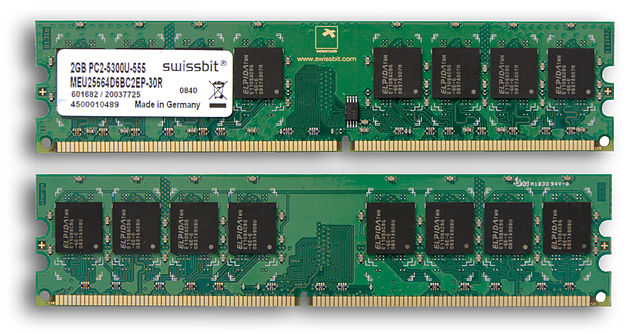
\includegraphics[scale=1.5]{chapters/chp3/images/Swissbit-2GB-PC2-5300U-555.jpg}
    \caption{Dois módulos de \acrshort{RAM} Swissbit\textsuperscript{\textregistered} 
    PC2-5300 DDR2 com capacidade de 2 Gigabytes, utilizada em computadores de mesa \cite{wiki:ddr2_ram}.}
    \label{fig:ram}
\end{figure}